\chapter{Tools di analisi}
\section{DDSFuzz}
DDSFuzz è un tool di analisi open source con l'obiettivo di 
effettuare test di tipo fuzz
in modo da testare vari input che il middleware DDS può
ricevere durante la sua esecuzione. Prima di questo strumento 
non esistevano (o non erano disponibili al pubblico) soluzioni
per effettuare questo tipo di test specifico per il DDS, mancanza
che questo tool cerca di colmare. Infatti anche se esistono tool 
come RoboFuzz e Deng et al, quest'ultimi vengono utilizzati 
per testare applicativi ROS (Robotic Operation System), che 
utilizzano solo una parte delle funzioni del DDS, tralasciando
così delle funzionalità del middleware che non vengono usufruite
da ROS.


\subsection{Fuzz testing}
Prima di parlare del tool DDSFuzz dobbiamo prima comprendere 
il significato di fuzzing (chiamato anche fuzz test) che è
alla base del funzionamento di questo tool. Il fuzzing è un test
automatizzato che serve a trovare e creare casi limite utilizzando
dati di input invalidi in modo tale da esplorare più vulnerabilità
possibili all'interno di un software. 
Inizialmente i primi tool di fuzzing non erano molto 
semplici da utilizzare o conosciuti, ma con il tempo questi strumenti
sono migliorati rendendoli più user-friendly aumentando così la 
loro frequenza di uso per testare softwares. I software che possono 
essere sottoposti a questo tipo di test possono essere 
di ogni tipo: compilatori, applicazioni, protocolli network 
e kernel \cite{8371326}.

\begin{figure}[H]
    \centering
    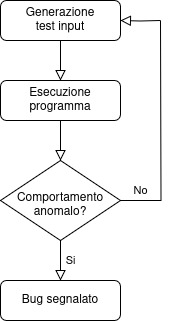
\includegraphics[width=5cm, keepaspectratio]{img/Diagramma di flusso fuzzer.jpg}
    \caption{Diagramma di flusso del funzionamento di un fuzzer.}
    \label{funzionamento fuzzer}
\end{figure}

Questi fuzzing test simulano un attacco mandando al software
che si vuole testare input regolari e irregolari, 
in modo tale da poter 
accedere ad ogni parte del codice con ogni tipo di input possibile.
In questo modo è possibile analizzare il comportamento del software
ed è possbile distinguere casi anomali o insicuri che non dovrebberò
essere possibili. Infatti quando questo test è attivo il fuzzer riceverà
varie informazioni riguardanti lo stato e l'output del programma, in 
modo tale da poter distiguere il suo comportamento. Se viene scoperto
qualche comportamento anomalo (ad esempio un segmentation fault) il 
fuzzer segnalerà in un log gli input utilizzati in modo tale da poter 
segnalare il bug.

Tuttavia dato che questi test sono generalizzati per essere compatibili
con vari software, si creà una sorta di imprecisione nel mandare i vari 
input. Questi input a volte non sono variegati a sufficienza 
per analizzare ogni singola parte del software che stiamo analizzando.
Inoltre in molti casi può anche succedere che vengono creati
dei test che non sono necessari consumando risorse e tempo inutilmente.

Per migliorare la qualità di questi test è stato 
creato il DDSFuzz che essendo un fuzzer specifico solamente per 
il middleware DDS rimuove molte delle imprecisioni di un fuzzer 
più generico.

\subsection{Funzionamento DDSFuzz}
DDSFuzz essendo specializzato per il DDS prende in considerazione 
molte sue caratteristiche che non sono presenti in altri software o 
altre tipologie di protocollo. La prima considerazione che viene 
effettuata da DDSFuzz è che durante l'esecuzione del middleware DDS 
la topologia della rete può mutare nel tempo creando problemi per 
fuzzer tradizionali che non si adattano ai cambiamenti. Infatti certi
dispositivi si possono connettere o disconnettere dalla rete a loro 
piacimento rendendo quindi necessario cambiare i vari input di test 
evitando ad esempio di trasmettere informazioni verso un'entità 
che si è disconnessa. DDSFuzz prende anche in considerazione le
policy QoS, applicate ad ogni entità, e 
le funzionalità abilitate dal DDS security, come
l'autenticazione e il controllo accessi, in modo tale da
poter creare test più accurati. 